% -*- TeX:de -*-
\NeedsTeXFormat{LaTeX2e}
\documentclass[12pt,a4paper]{article}
\usepackage[german]{babel} % german text
\usepackage[DIV12]{typearea} % size of printable area
\usepackage[T1]{fontenc} % font encoding
%\usepackage[latin1]{inputenc} % most likely on Windows
\usepackage[utf8]{inputenc} % probably on Linux
\usepackage{multicol}

% PLOTTING
\usepackage{pgfplots} 
\usepackage{pgfplotstable}
\usepackage{url}
\usepackage{graphicx} % to include images
\usepackage{tikz}
\usepackage{subfigure} % for creating subfigures
\usepackage{amsmath} % a bunch of symbols
\usepackage{amssymb} % even more symbols
\usepackage{booktabs} % pretty tables
\usepackage{makecell} % multi row table heading

% a floating environment for circuits
\usepackage{float}
\usepackage{caption}

%\newfloat{circuit}{tbph}{circuits}
%\floatname{circuit}{Schaltplan}

% a floating environment for diagrams
%\newfloat{diagram}{tbph}{diagrams}
%\floatname{diagram}{Diagramm}

\selectlanguage{german} % use german

\begin{document}

%%%%%%% DECKBLATT %%%%%%%
\thispagestyle{empty}
			\begin{center}
			\Large{Fakultät für Physik}\\
			\end{center}
\begin{verbatim}


\end{verbatim}
							%Eintrag des Wintersemesters
			\begin{center}
			\textbf{\LARGE WS 2013/14}
			\end{center}
\begin{verbatim}


\end{verbatim}
			\begin{center}
			\textbf{\LARGE{Physikalisches Praktikum\\ für das Bachelorstudium}}
			\end{center}
\begin{verbatim}




\end{verbatim}

			\begin{center}
			\textbf{\LARGE{PROTOKOLL}}
			\end{center}
			
\begin{verbatim}

\end{verbatim}

			\begin{flushleft}
			\textbf{\Large{Experiment (Nr., Titel):}}\\
							%Experiment Nr. und Titel statt den Punkten eintragen
			\LARGE{PW9 Gleichstrom}	
			\end{flushleft}

\begin{verbatim}

\end{verbatim}	
							%Eintragen des Abgabedatums, oder des Erstelldatums des Protokolls
			\begin{flushleft}
			\textbf{\Large{Datum:}} \Large{21.11.2013}
			\end{flushleft}
			
\begin{verbatim}
\end{verbatim}
							%Namen der Protokollschreiber
		\begin{flushleft}
			\textbf{\Large{Namen:}} \Large{Patrick Braun, Johannes Kurz}
			\end{flushleft}

\begin{verbatim}


\end{verbatim}
							%Kurstag und Gruppennummer, zb. Fr/5
			\begin{flushleft}
			\textbf{\Large{Kurstag/Gruppe:}} \Large{DO/2}
			\end{flushleft}

\begin{verbatim}

\end{verbatim}
							%Name des Betreuers, das Praktikum betreute.
			\begin{flushleft}
			\LARGE{\textbf{Betreuer:}}	\Large{ Clemens Nagel }	
			\end{flushleft}

%%%%%%% DECKBLATT ENDE %%%%%%%
\pagebreak
\setlength{\columnsep}{20pt}
\begin{multicols}{2}

%%%%%%%%%%%%%%%%%%%%%%%%%%%%%%%%%%%%%%%%%%%%%%%%
%\end{multicols}
%\begin{figure}[H]
%	\centering
%	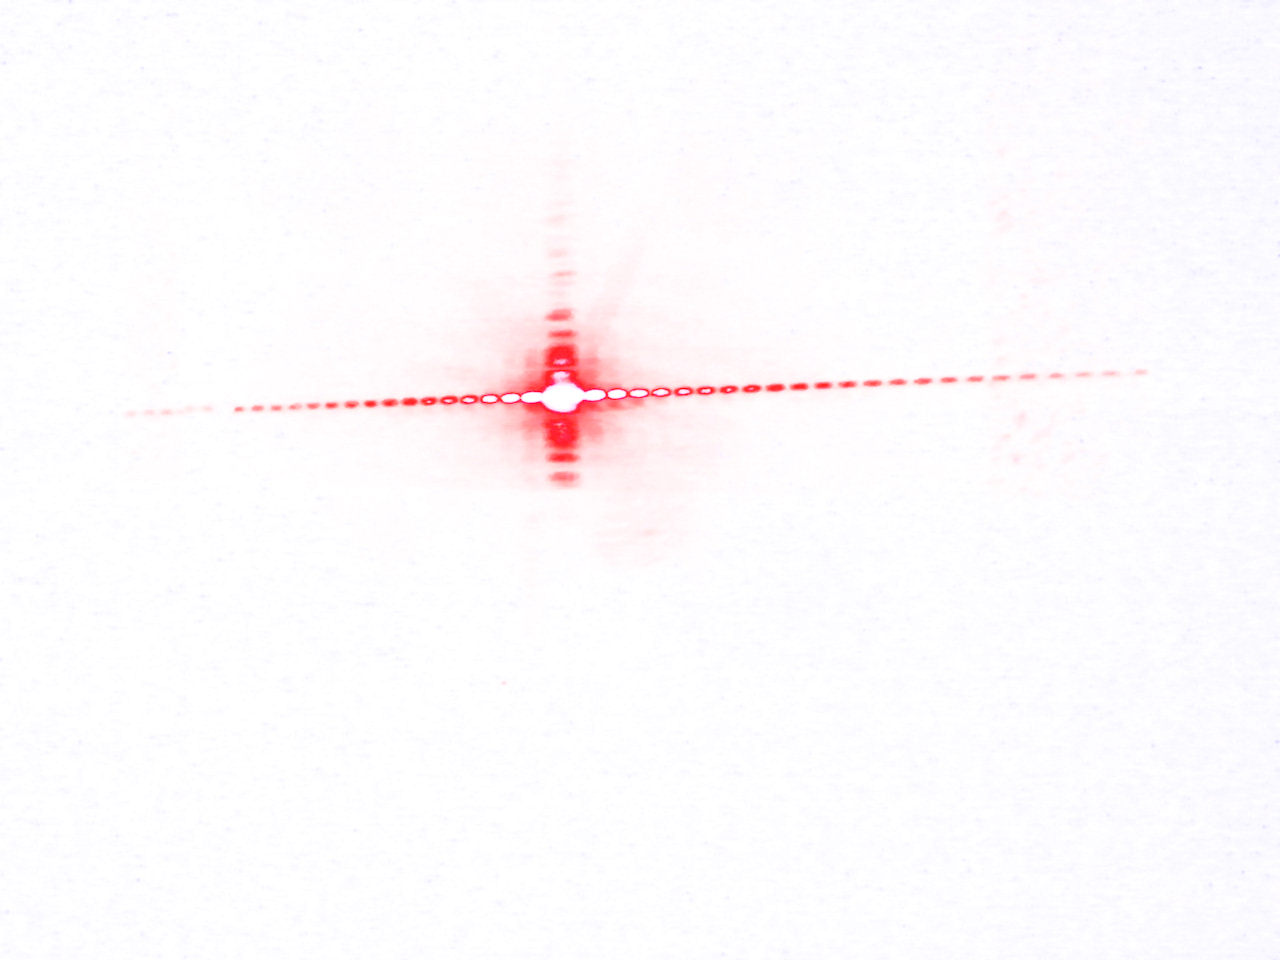
\includegraphics[scale=0.35]{./figure/beugung.png}
%	\caption{Beugungsmuster Einzelspalt (echtes Foto; schwarz durch weiß ersetzt)}
%	\label{fig:beugungsmuster}
%\end{figure}


%\begin{figure}[H]
%	\centering
%	\pgfplotstabletypeset[
%			columns={abstand, n},
%			col sep=&,
%			columns/abstand/.style={precision=2, zerofill, column name=\makecell{$Abstand$\\$(\pm 0.05)[mm]$} }, 
%			columns/n/.style={column name=\makecell{$n$\\$(Ordnung)$}, precision=0},
%			every head row/.style={before row=\hline,after row=\hline\hline},
%			every last row/.style={after row=\hline},
%			every first column/.style={column type/.add={|}{} },
%			every last column/.style={column type/.add={}{|} }
%			]{
%			abstand & n
%			12.9 & 1
%			24.45 & 2
%			37.40 & 3
%			49.35& 4
%			62.45 & 5
%			74.45 & 6
%			87.45 & 7
%			100.25 & 8
%			
%			}
%	\caption{Messwerte Einzelspalt}
%	\label{tab:werte_einzelspalt}
%\end{figure}
%


\section{Photovoltaische Solarzellen als Gleichstromquelle}
In diesem Experiment wird eine Solarzelle auf ihre Eigenschaften bei einer bestimmten Lichtintensität untersucht. Zu diesem Zweck wird eine Lampe in einem gewissen Abstand über einer Solarzelle befestigt. Bei konstantem Abstand und konstanter Lichtintensität kann mit einem regelbarem Widerstand (Abb. \ref{fig:schaltbild_solarzelle} $R_L$) eine Messreihe durchgeführt werden. Ziel ist es, die Werte für $I_{KS}$ den Kurzschlussstrom und $U_{LL}$ die Leerlaufspannung zu extrapolieren. \\
\begin{figure}[H]
	\centering
	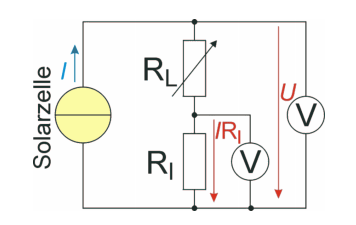
\includegraphics[scale=0.6]{./figure/solarzelle_schaltplan.png}
	\caption{Schaltplan zur Bestimmung der Strom-Spannungskennlinie$^{[1]}$}
	\label{fig:schaltbild_solarzelle}
\end{figure}
\noindent
In Abbildung \ref{fig:schaltbild_solarzelle} ist der Aufbau ersichtlich. Durch Messung der Klemmenspannung ($I * R_I$) und der Gesamtspannung ($U$) lässt sich die Schaltung und somit die Solarzelle beschreiben.\\
Trägt man die Werte in einem U-I-Diagramm auf, erhält man die Strom-Spannungskennline der Solarzelle. Weiters kann über ein $\Omega-P$-Diagramm der Punkt der maximalen Leistung $P_{max}$ ermittelt werden.\\
Zuletzt wird der Kurvenfüllfaktor CFF über folgende Beziehung errechnet:
$$CFF = \frac{P_{max}}{I_{KS}*U_{LL}}$$
Der CFF-Wert bestimmt das Sprungverhalten von Spannung zu Leerlaufspannung. Bei einem Wert von CFF = 1 springt die Kurve ideal. Bei derzeitigen Optimierungen kann ein Wert von 0.8 - 0.9 erreicht werden.\\
Für die Berechnung des Stroms wird das Ohmsche Gesetzt verwendet:
$$I = \frac{U_{gemessen}}{R_I}$$
wobei $R_I$ in [1](1.3) gegeben ist.
\subsection{Messwerte und Ergebnisse}
\end{multicols}
\begin{figure}[H]
	\centering
	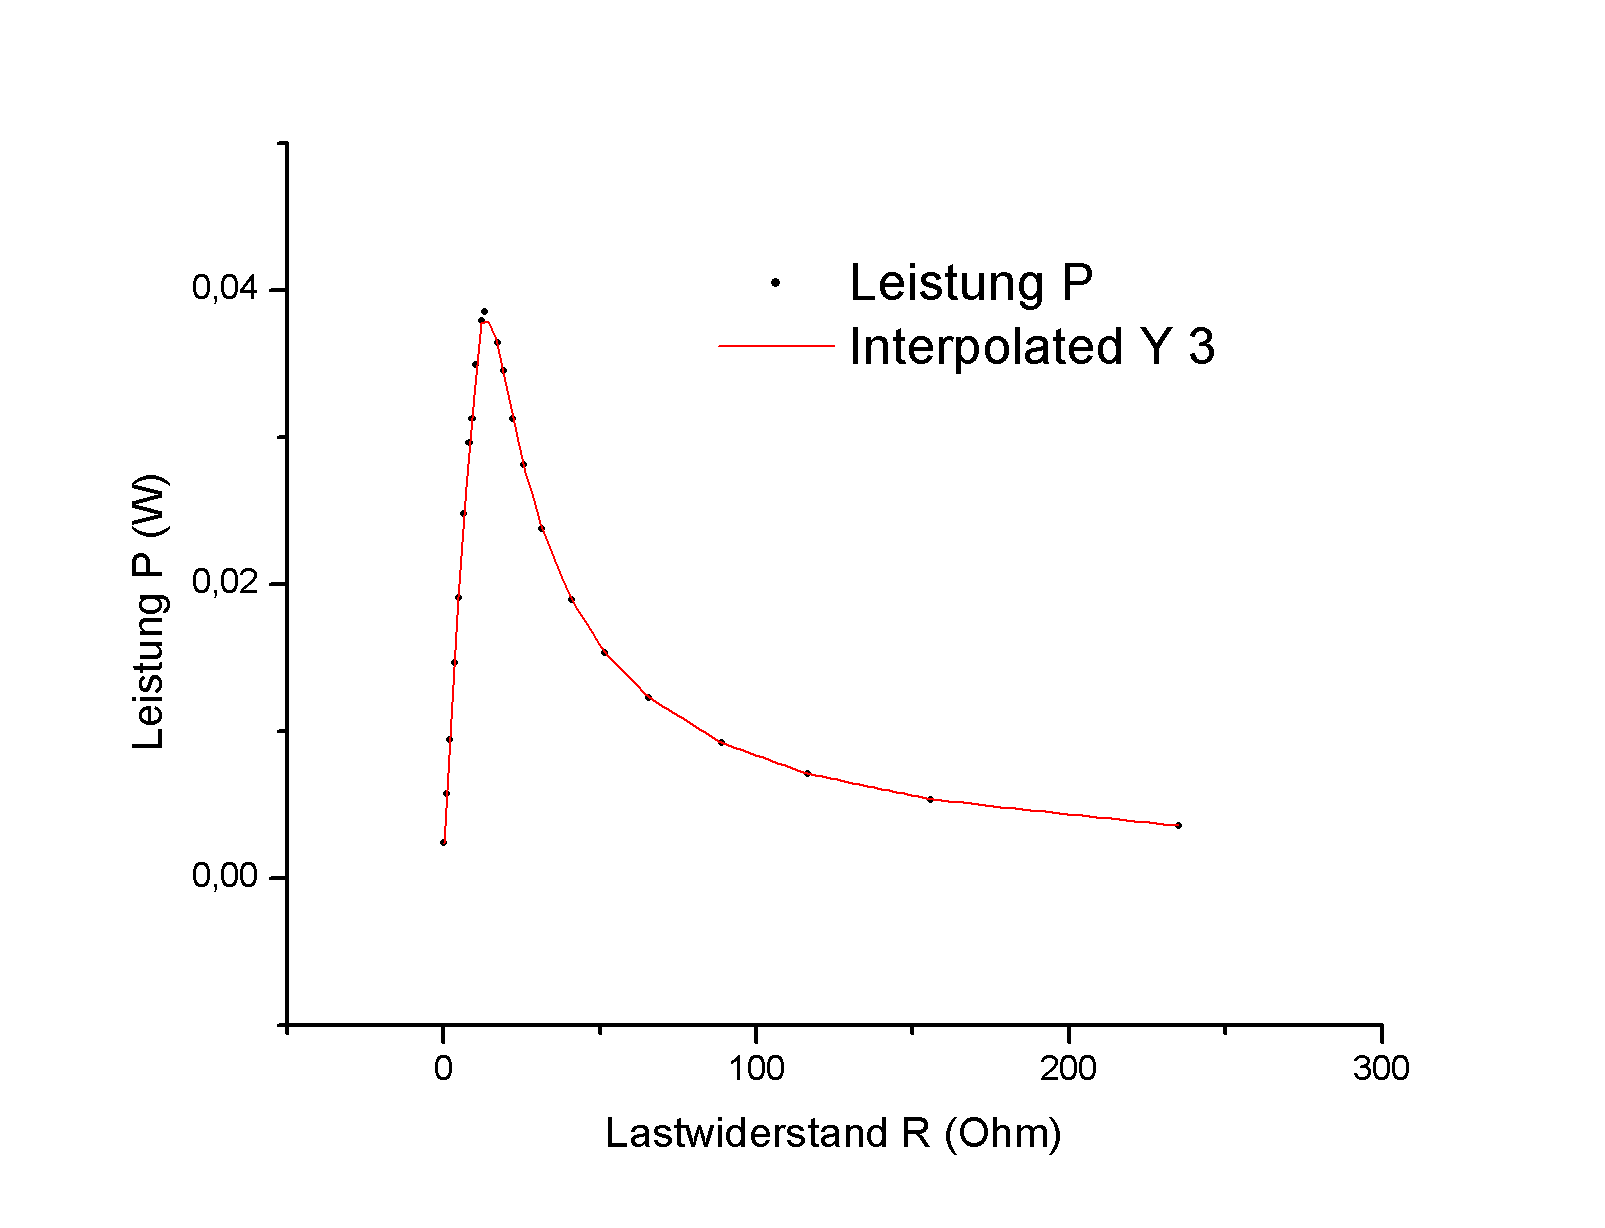
\includegraphics[scale=0.6]{./figure/solarzelle_pmax.png}
	\caption{Widerstand gegen Leistung; $P_{max}$}
	\label{fig:solarzelle_leistung}
\end{figure}
\begin{multicols}{2}
\noindent
Abstand zwischen Lichtquelle und Solarzelle:
$$l = 20cm$$
Werte mit SE-Mean:
$$I_{KS} = (61.58 \pm 1.99) mA$$
$$U_{LL} = (927.27 \pm 0.01) mV$$
$$P_{max} = (38.51 \pm 0.88) mW$$
$$CFF = 0.6744$$

\end{multicols}
\begin{figure}[H]
	\centering
	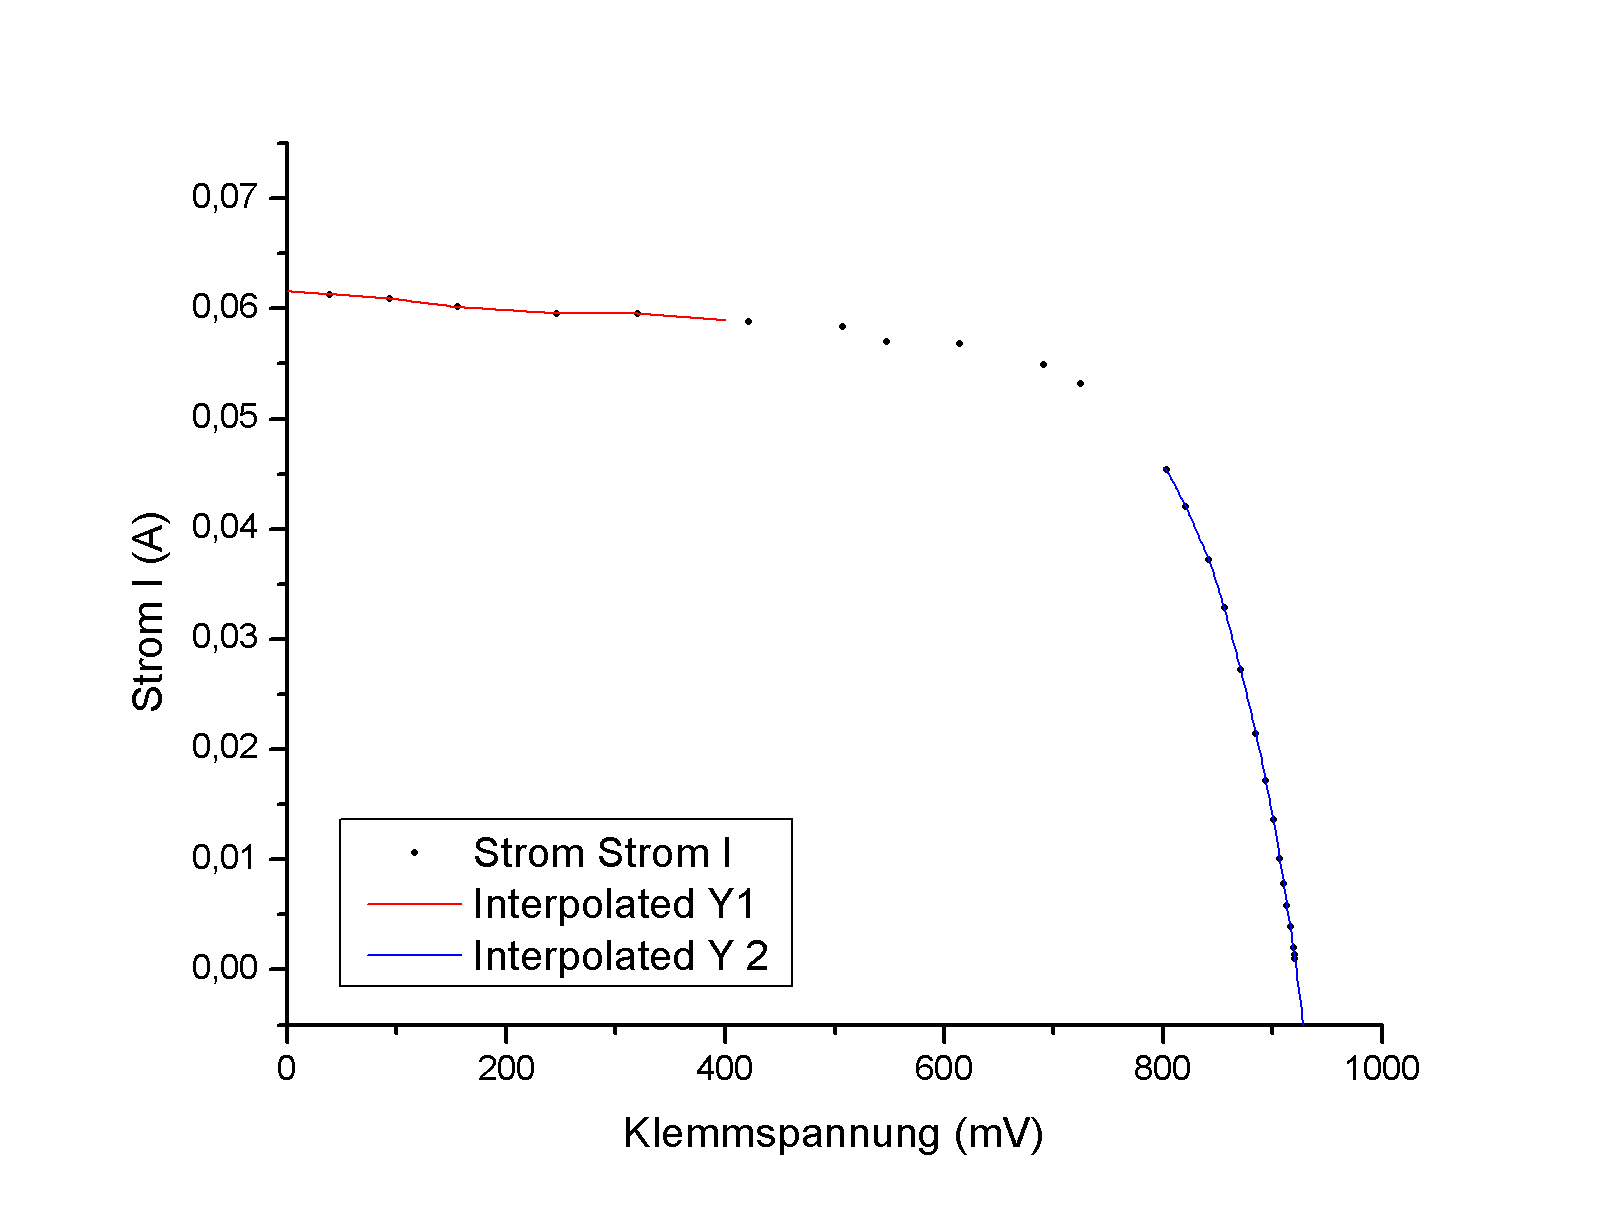
\includegraphics[scale=0.6]{./figure/solarzelle_strom_spannung.png}
	\caption{Spannung gegen Strom; Kennlinie}
	\label{fig:solarzelle_strom_spannung}
\end{figure}

\begin{multicols}{2}

\subsection{Diskussion}
Der Aufbau und  die Messung der Spannungen gestaltete sich dank zweier Fluke Messgeräte unproblematisch. Zu beachten war nur der korrekte Messbereich und das Umschalten auf Gleichstrom. Mit dem Schaltplan \ref{fig:schaltbild_solarzelle} ist der Aufbau bis auf den regelbaren (durch Drehung) Widerstand vollständig erklärt. \\
Beim regelbaren Widerstand musste vorsichtig gedreht werden und dabei auf den jeweiligen Anstieg bzw. Abfall wie in [1] (1.3) beschrieben zu achten. Bei der Auswertung wurde für die Berechnung der Werte $I_{KS}$ und $U_{LL}$ mit Origin 9 jeweils eine Interpolation in einem glatten Kurvenbereich durchgeführt. Für $U_{LL}$ ist der Fehler der interpolierten Werte mit 
$(0.0000774322) mV$ so gering das die Anzeigegenauigkeit der Messgeräte herangezogen wurde ($\pm 0.01mV$).\\
Bei der Interpolation für den Kurzschlussstrom $I_{KS}$ ergab sich durch die in \ref{fig:solarzelle_strom_spannung} ersichtlichen Knicke in der roten Kurve ein weit größerer Fehler. Die Ungenauigkeit könnte durch zu schnelle Messvorgänge hintereinander entstanden sein.\\
Der Kurvenfüllfaktor CFF liegt mit 0.6744 etwas unter den technisch machbaren Werten von 0.8-0.9. Dieser Wert kann aber als korrekt gewertet werden, da die blaue Kurve in \ref{fig:solarzelle_strom_spannung} einen runden Verlauf hat. Optimal wäre ein (fast) gerader Abfall.\\
Bei der Berechnung der Maximalen Leistung $P_{max}$ wurde ebenfalls eine Interpolation durchgeführt und beim Maximum eine punktuelle Koordinatenablesung durchgeführt.\\


%%%%%%%%%%%%%%%%%%%%%%%%%%%%%%%%%%%%%%%%%%%%%%%%
\section{Widerstandsbestimmung mittel Wheatstone-Brücke}

Eine Möglichkeit, einen Widerstand zu messen, ohne mit 2 Messgeräten (und 2 Messunsicherheiten) Spannung und Strom zu bestimmen ist eine Wheatstone-Brückenschaltung.
\\
Der zu messende Widerstand (hier $R_x$) und 3 andere werden, paarweise parallel geschaltet, und innerhalb beider Zweige in Serie. 

Die beiden Zweige der Parallelschaltung werden durch ein Voltmeter verbunden, wie in Abb. \ref{fig:wheatstone_schaltplan} skizziert.



\begin{figure}[H]
	\centering
	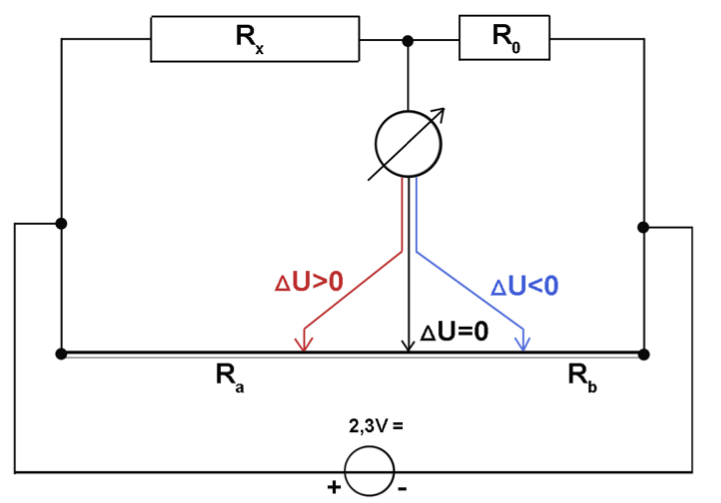
\includegraphics[scale=0.50]{./figure/wheatstone_schaltplan.png}
	\caption{Schaltskizze einer Wheatstonebrücke}
	\label{fig:wheatstone_schaltplan}
\end{figure}

An beiden Zweigen der Parallelschaltung liegt die gleiche Spannung an (Kirchhoff Schleifenregel). Diese teilt sich an den in Serie geschalteten Widerständen in derem Verhältnis auf.\\
Die Spannung im Messgerät (Indikatorzweig) verschwindet genau dann, wenn die Verhältnisse der Widerstände an beiden Brückenzweigen gleich sind.

$$\frac{R_x}{R_0} = \frac{R_a}{R_b}$$
$$\Rightarrow R_x = R_0 \cdot \frac{R_a}{R_b}$$

Es genügt also, $R_0$ zu kennen, sowie das Verhältnis von $R_a$ zu $R_b$. Ihre Widerstandswerte sind nicht von Bedeutung.\\
\\
In diesem Versuch werden die WIderstände $R_a$,$R_b$ durch einen Draht realisiert, der an einer Längenskala befestigt ist, an der auch ein beweglicher Schleifer montiert ist. Durch diesen wird wird die Unterteilung in 2 Widerstände erzeugt (das Voltmeter ist am Schleifer angeschlossen).
\\
Da der Draht über die ganze Länge die gleiche Dicke hat, ist der Widerstand pro Längeneinheit überall gleich. Somit ist das Verhältnis der Drahtstücke, die durch den Schleifer getrennt werden gleichzeitig das Verhältnis der Widerstände.\\
Als $R_0$ wird eine Widerstandsdekade verwendet, auf der sich, in diskreten Schritten, Widerstände in von 1$ \Omega$ bis 10M$\Omega$ einstellen lassen
\\
Der Schleifer wird so lange verrückt, bis am Messgerät keine Spannung anliegt. Dann sind die Spannungsverhältnisse in beiden Zweigen gleich und der gesuchte Widerstand kann berechnet werden.\\
Es ist dabei eigentlich nicht notwendig, die Widerstandsdekade anders einzustellen. In der Diskussion wird jedoch näher erklärt, warum es sinnvoll ist, nicht das $R_a$-$R_b$-Verhältnis zu ändern, sondern $R_0$ anzupassen.

\subsection{Messwerte und Ergebnisse}


$$R_G = (1200 \pm 13) \Omega$$
$$R_F = (324 \pm 3.5) \Omega$$
$$R_F = (6900 \pm 75) \Omega$$
\\

\noindent Ergebnisse für $R_G$ und $R_F$ aus ersten Testmessungen, ohne Optimierung der Methode:
\\
$R_{G1} = (1290 \pm 23) \Omega$, $\frac{R_a}{R_b}=\frac{946}{54}$\\
$R_{G2} = (1193\pm 13) \Omega$, $\frac{R_a}{R_b}=\frac{423}{576}$\\
\\
$R_{F1} = (330 \pm 7) \Omega$, $\frac{R_a}{R_b}=\frac{782}{218}$\\
$R_{F2} = (318\pm 7) \Omega$, $\frac{R_a}{R_b}=\frac{182}{818}$\\

\subsection{Diskussion}

Erste Messungen wurden durchgeführt, indem, bei zufällig (grob geschätzt) eingestelltem $R_0$ das Ausgleichsverhältnis nur am Schiebewiderstandssystem eingestellt wurde.\\
Das führt beispielsweise für $R_{G1}$ zu einem Verhältnis der Spannungen in beiden Zweigen von beinahe 20:1.\\
In der zweiten Messung ($R_{G2}$) wurde das Verhältnis so gewählt, dass der Schleifer fast auf Mittelstellung ist, und damit $R_a$/$R_b$ beinahe 1 ist.\\
Es sollten zuerst nur die Unsicherheiten betrachtet werden: Diejenige von $R_{G1}$ ist beinahe doppelt so groß, wie die von $R_{G2}$ (oder auch $R_G$):\\
Es wurde jeweils die Unsicherheit der Widerstandsdekade mit 1\% vom eingestellten Wert angenommen (Herstellerangabe [2]) und die Längenskala mit $\pm$ 1 (von 1000 Skalenstrichen). Das entspricht ihrer Auflösung (lsd), da davon ausgegangen werden kann, dass die Eich- und Linearitätsunsicherheit davon schon gecovert werden.\\
Liegen nun $R_a$ und $R_b$ weit auseinander, ist die relative Unsicherheit durch den größeren Längenabschnitt zwar eher klein, am kürzeren Längenabschnitt jedoch groß.\\
Da die Digitalisierungs-Unsicherheiten beider Längen korrelieren (ist einer zu groß, muss der andere zu klein sein und umgekehrt), lassen sich hier noch kleine Optimierungen in der Rechnung durchführen, der Effekt ist aber nicht so groß im Vergleich mit dem des Ungleichgewichts.\\
Die günstigste Position ist daher die Mitte, also ein 1:1 Verhältnis der Widerstände an beiden Zweigen. Hier zeigt sich auch der tiefere Sinn des Aufbaus mit der Widerstandsdekade anstatt eines festen $R_0$:
\\
Die beiden Schiebewiderstände werden genau auf Mittelstellung gebracht, und das Gleichgewicht am Indikatorzweig wird durch Veränderung von $R_0$ erzeugt. Auf diese Art wurden letztendlich alle 3 Widerstände gemessen. Gut zu erkennen an den Ergebnissen ist, dass die Unsicherheiten jeweils im Wesentlichen den 1\% von der Widerstandsdekade entsprechen.
\\
\\
Diese Methode hat bietet noch zusätzliche Vorteile:\\
Das Ergebnis kann direkt an der Dekade abgelesen werden, da ja $R_x$ gleich $R_0$ sein muss. Dadurch lassen sich mehrere Widerstände schneller messen und die Fehlerrechnung schneller durchführen ($R_a$/$R_b$ ist jetzt eine Konstante mit fester Unsicherheit).\\
Der Schleifer wäre ersetzbar durch 2 gleiche, fixe, Widerstände. Das würde eventuelle systematische Fehler durch den Schleifkontakt und mangelnde Drahtspannung sowie seiner Aufhängung, beseitigen.\\
\\
Zuletzt soll noch der Messwert $R_{G1}$ betrachtet werden: Hier dürfte ein Messfehler passiert sein, da der Wert, trotz großer Unsicherheit weit außerhalb des erwarteten Bereichs liegt. Da insgesamt jedoch zu wenig Messungen vorliegen, lässt sich keine genauere Aussage machen, ob nicht dieser Wert näher am wahren Wert liegt.\\
Da jedoch die anderen beiden Messungen gut beieinander liegen und auch die Testmessungen für $R_F$ seine finale Messung bestärken (die mit der gleichen Schiebereinstellung, wie die finale $R_G$
-Messung durchgeführt wurde), ist es wahrscheinlich, dass $R_{G1}$ falsch gemessen wurde.\\
\\
Ob dabei die Präzision des Aufbaus mit dem Draht und dem Schleifer so einen großen Effekt haben ist fraglich, und müsste ausführlicher überprüft werden. Ein einfacher Ablesefehler an der Dekade ist denkbar.

%%%%%%%%%%%%%%%%%%%%%%%%%%%%%%%%%%%%%%%%%%%%%%%%
\section{Reale Spannungsquelle}
In diesem Versuch soll der Innenwiderstand $R_i$ einer Batterie gemessen werden.\\
Der Innenwiderstand ist ein Ohmscher Widerstand, der konstruktionsbedingt schon vor den Kontakten der Spannungsquelle zum Rest des Stromkreises auftritt. Ideale Spannungsquellen (deren Innenwiderstand = 0) lassen sich real nicht bauen, da ja schon jede beliebig kurze Leiterstrecke einen Widerstand darstellt.\\
Dieser Umstand kann in einem Ersatzschaltbild dargestellt werden, in dem die reale Spannungsquelle als eine ideale, mit dem Innenwiderstand $R_i$ in Serie geschaltet, eingezeichnet wird:



\begin{figure}[H]
	\centering
	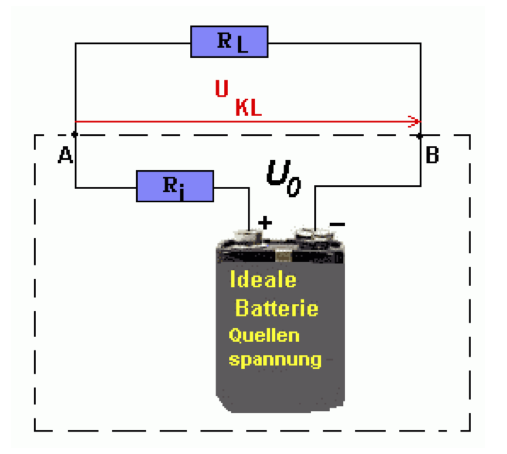
\includegraphics[scale=0.80]{./figure/innenwiderstand_schaltskizze.png}
	\caption{Ersatzschaltbild einer realen Spannungsquelle mit Verbraucher}
	\label{fig:innenwiderstand_schaltskizze}
\end{figure}

Es gilt also nach Kirchhoff:
$$U-0 = (R_i + R_L) \cdot I = U_i + U_L$$
Im Versuch messbar sind die Spannung $U_L$ am Verbraucher sowie der Strom, der in der Serienschaltung überall gleich sein muss.
$$U_L = U_0 - R_i \cdot I$$
Das entspricht, trägt man $U_L$ gegen $I$ in einem Diagramm auf,  einer Geradengleichung mit $U_0$ als y-Achsenabschnitt und -$R_i$ als Steigung.
Die Spannung $U_L $ zwischen den Punkten A und B wird mit einem Voltmeter gemessen, der Strom $I$ mit dem Amperemeter zwischen A und dem Lastwiderstand $R_L$ (Abb. \ref{fig:innenwiderstand_schaltskizze}). Dieser wird im Versuch durch die Widerstandsdekade aus der Wheatstone-Messung realisiert.\\
Zuerst wird die Leerlaufspannung der Batterie gemessen.\\
Beginnend bei 200$\Omega $ werden an allen 10$\Omega$-Schritten Messungen durchgeführt, die letzte bei 15$\Omega$. Durch linearen Fit werden $U_0$ und $R_i$ bestimmt.\\
Es ist darauf zu achten, den Stromkreis nur zur Messung zu schließen, und zwischen den Messungen kurze Pausen zu lassen, damit sich die Spannung stabilisiert.


\end{multicols}
\subsection{Messwerte und Ergebnisse}
\textbf{$U_L$ wurde gemessen:}





% Batterie ohne Fit... gemessen

\begin{figure}[H]
	\centering
	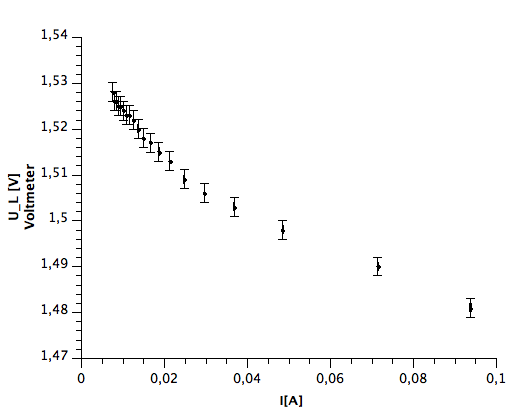
\includegraphics[scale=0.58]{./figure/Batterie_UI_ohneFit.png}
	\caption{Spannung/Strom-Diagramm; gemessene Spannungen}
	\label{fig:Batterie_UI_ohneFit}
\end{figure}


% Batterie mit Fit... gemessen, bereich

\begin{figure}[H]
	\centering
	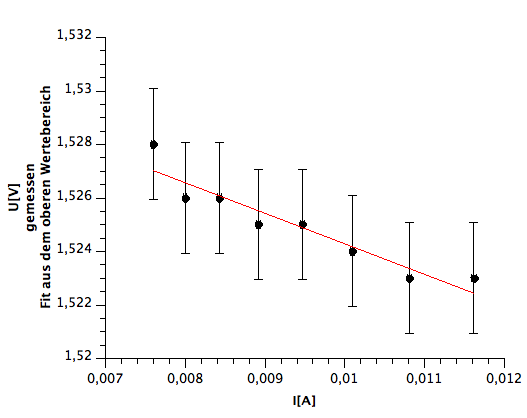
\includegraphics[scale=0.58]{./figure/Batterie_UI_mitFit_Abschnitt.png}
	\caption{Spannung/Strom-Diagramm; gemessene Spannungen - \\
	Ausschnitt aus dem oberen Wertebereich}
	\label{fig:Batterie_UI_mitFit_Abschnitt}
\end{figure}




\textbf{$U_L$ wurde aus $R_L$*I berechnet:}

% Batterie gerechnet mit fit


\begin{figure}[H]
	\centering
	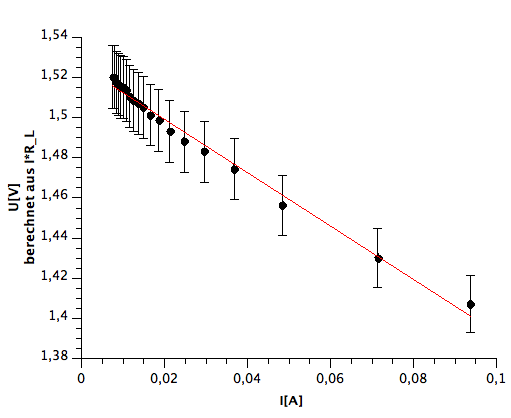
\includegraphics[scale=0.58]{./figure/Batterie_RI-I_mitFit.png}
	\caption{Spannung/Strom-Diagramm; berechnete Spannungen}
	\label{fig:Batterie_RI-I_mitFit}
\end{figure}

% Batterie gerechnet mit fit, bereich


\begin{figure}[H]
	\centering
	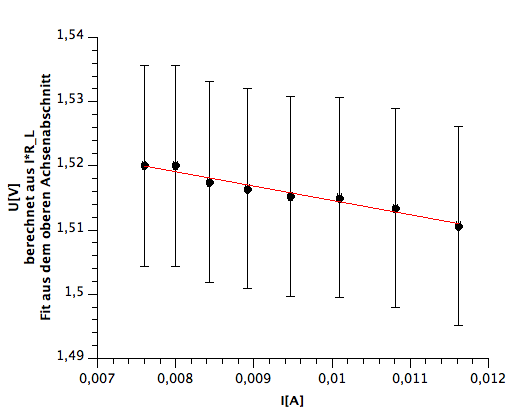
\includegraphics[scale=0.58]{./figure/Batterie_RI-I_mitFit_Abschnitt.png}
	\caption{Spannung/Strom-Diagramm; berechnete Spannungen  - \\
	Ausschnitt aus dem oberen Wertebereich}
	\label{fig:Batterie_RI-I_mitFit_Abschnitt}
\end{figure}




\begin{multicols}{2}


\begin{itemize}

	\item
	%% bereich aus UL
	\noindent aus dem Fit in Abb. \ref{fig:Batterie_UI_mitFit_Abschnitt}:
	$$U_0=(1535.7 \pm 53)mV$$
	$$R_i=(1.14 \pm 0.56)\Omega$$
	(Fit über einen \textbf{Teilbereich} aus den \textbf{gemessenen} Daten)\\
	
	
	
	\item
	%% alles aus R*I
	\noindent aus dem Fit in Abb. \ref{Spannung/Strom-Diagramm; berechnete Spannungen}:
	$$U_0 = (1527.8 \pm 1.1)mV$$
	$$R_i=(0.551 \pm 0.032)m \Omega$$
	(Fit über einen \textbf{gesamten Bereich} aus den \textbf{berechneten} Daten)\\
	
	
	\item
	\noindent aus dem Fit in Abb. \ref{fig:Batterie_RI-I_mitFit_Abschnitt}:
	%% bereich aus R*I
	$$U_0=(1537 \pm 40)mV$$
	$$R_i=(2.2 \pm 4.3)\Omega$$
	(Fit über einen \textbf{Teilbereich} aus den \textbf{berechneten} Daten)\\
	\\
	\\
\end{itemize}

\noindent gemessene Leerlaufspannung:\\
$U_{Leerlauf}=(1.537 \pm 0.002)V$

\subsection{Diskussion}
In der Betrachtung der Ergebnisse fallen sofort 2 große Abweichungen von der Theorie auf:\\
\begin{itemize}
	\item Die Punkte bilden keine Gerade
	\item Die berechneten Quellenspannungen sind tendentiell niedriger als die gemessenen Leerlaufspannungen
\end{itemize}

\noindent Das Problem mit der Quellenspannung, die ja aus dem y-Achsenabschnitt des Fits gelesen wird, ist vermutlich eine Folge des ersten Problems, dass hier keine wirklich lineare Kurve vorliegt, und kann daher aus den gemessenen Daten nicht gesondert behandelt werden.\\
Der Effekt wurde jedoch als Indikator verwendet, dafür wie geeignet eine ermittelte Gerade als Aussage über das System sei: Beide Geraden, die nur durch einen Teil der Punkte gelegt wurden (denjenigen mit den höheren Klemmspannungen) ergeben Quellspannungen die, im Unsicherheitsbereich, plausibel sind.\\
(Dabei wurde in Abb.\ref{fig:Batterie_UI_ohneFit} gar keine Gerade durch den gesamten Datensatz mit den gemessenen Spannungen gelegt, da das zu keiner sinnvollen Aussage führt.)\\
Es scheint sich also, bei großen Strömen und kleinen Spannungen, eine Verzerrung der Kennlinie zu ergeben.\\
(In der Anleitung ist angegeben, dass dies bei kleinen Strömen der Fall sei. Fits durch den linearen Anteil bei großen Strömen ergeben jedoch unplausible Quellenspannungen, da diese nicht kleiner als die Leerlaufspannung sein können.)
\\
Interessant ist auch, dass das Diagramm, in dem die Spannung aus dem gemessenen Strom und den (durch die Widerstandsdekade bekannten) Lastwiderstand $R_L$ berechnet wurde (Abb. \ref{fig:Batterie_RI-I_mitFit}) einen lineareren Verlauf zeigt, als dasjenige in dem Spannung und Strom gemessen wurden.\\
(Die Daten stammen aus der gleichen Messung, es wurde also nicht einmal ein Multimeter aus dem Stromkreis entfernt. Der Einfluss des Voltmeters sollte ohnehin vernachlässigbar klein sein.)\\
Prinzipiell lässt sich also das Experiment auch mit nur einem Messgerät durchführen (bei bekannten Lastwiderständen), in diesem speziellen Fall (mit dem Indikator Quellenspannung $U_0$) scheint jedoch das Ergebnis aus dem oberen \textbf{Teilbereich} der \textbf{gemessenen} Daten am plausibelsten.\\
\\
Wird $U_L$ berechnet ergibt sich eine sehr viel größere Unsicherheit (Unsicherheit von $R_L$ und I, wobei das Amperemeter unsicherer ist, als das Voltmeter), als durch die Messungen. Das drückt sich vor allem in einem unbrauchbaren Ergebnis für $R_i$ aus den \textbf{berechneten} Daten aus einem 
\textbf{Teilbereich} aus (Abb. \ref{fig:Batterie_RI-I_mitFit_Abschnitt}). Der Verlauf der Daten ist annähernd linear, die großen Unsicherheiten erlauben jedoch verschiedenste Steigungen.\\
\\
Es erscheint also das Ergebnis aus einem Teilbereich der gemessenen Daten am plausibelsten:\\
\noindent aus dem Fit in Abb. \ref{fig:Batterie_UI_mitFit_Abschnitt}:
	$$U_0=(1535.7 \pm 53)mV$$
	$$R_i=(1.14 \pm 0.56)\Omega$$
	
Ohne weitere Behandlung der möglichen Fehler, die bei der Durchführung begangen wurden, Erweiterung der Theorie (nichtlineare Kennlinie der Dekade, Temperatur im System, instabile Batterie), oder mehrmaliger Durchführung und Analyse, lassen diese Ergebnisse keine zufriedenstellende Aussage über Quellenspannung und Innenwiderstand der Batterie zu.

%%%%%%%%%%%%%%%%%%%%%%%%%%%%%%%%%%%%%%%%%%

\section{Belasteter Spannungsteiler}
In diesem Experiment sollen 
\begin{figure}[H]
	\centering
	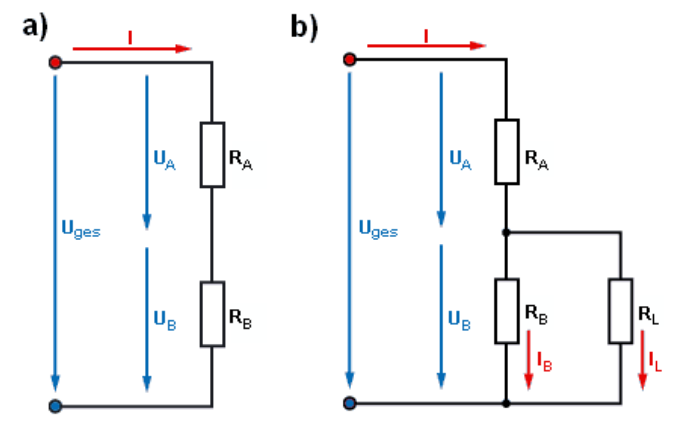
\includegraphics[scale=0.4]{./figure/spannungsteiler_schaltplan.png}
	\caption{Schaltplan Spannungsteiler a) unbelastet b) belastet$^{[1]}$}
	\label{fig:schaltbild_solarzelle}
\end{figure}
\noindent

\subsection{Messwerte und Ergebnisse}



\subsection{Diskussion}

%%%%%%%%%%%%%%%%%%%%%%%%%%%%%%%%%%%%%%%%%%


\section{Quellen}
$[1]$ Leitfaden, \url{http://www.univie.ac.at/anfpra/neu1/pw/pw9/PW9.pdf}\\
$[2]$ Widerstandsdekade Cosinus R1-3000, \url{http://www.farnell.com/datasheets/13334.pdf}\\

\end{multicols}


\end{document}